%%%%%%%%%%%%%%%%%%%%%%%%%%%%%%%%%%%%%%%%%
% Short Sectioned Assignment
% LaTeX Template
% Version 1.0 (5/5/12)
%
% This template has been downloaded from:
% http://www.LaTeXTemplates.com
%
% Original author:
% Frits Wenneker (http://www.howtotex.com)
%
% License:
% CC BY-NC-SA 3.0 (http://creativecommons.org/licenses/by-nc-sa/3.0/)
%
%%%%%%%%%%%%%%%%%%%%%%%%%%%%%%%%%%%%%%%%%

%----------------------------------------------------------------------------------------
%	PACKAGES AND OTHER DOCUMENT CONFIGURATIONS
%----------------------------------------------------------------------------------------

\documentclass[paper=a4, fontsize=11pt]{scrartcl} % A4 paper and 11pt font size
\usepackage[utf8]{inputenc}
\usepackage[T1]{fontenc} % Use 8-bit encoding that has 256 glyphs
\usepackage{fourier} % Use the Adobe Utopia font for the document - comment this line to return to the LaTeX default
\usepackage[english,croatian]{babel} % English language/hyphenation
\usepackage{amsmath,amsfonts,amsthm} % Math packages

\usepackage{lipsum} % Used for inserting dummy 'Lorem ipsum' text into the template

\usepackage{sectsty} % Allows customizing section commands
\allsectionsfont{\centering \normalfont\scshape} % Make all sections centered, the default font and small caps

\usepackage{fancyhdr} % Custom headers and footers
\pagestyle{fancyplain} % Makes all pages in the document conform to the custom headers and footers
\fancyhead{} % No page header - if you want one, create it in the same way as the footers below
\fancyfoot[L]{} % Empty left footer
\fancyfoot[C]{} % Empty center footer
\fancyfoot[R]{\thepage} % Page numbering for right footer
\renewcommand{\headrulewidth}{0pt} % Remove header underlines
\renewcommand{\footrulewidth}{0pt} % Remove footer underlines
\setlength{\headheight}{13.6pt} % Customize the height of the header

\numberwithin{equation}{section} % Number equations within sections (i.e. 1.1, 1.2, 2.1, 2.2 instead of 1, 2, 3, 4)
\numberwithin{figure}{section} % Number figures within sections (i.e. 1.1, 1.2, 2.1, 2.2 instead of 1, 2, 3, 4)
\numberwithin{table}{section} % Number tables within sections (i.e. 1.1, 1.2, 2.1, 2.2 instead of 1, 2, 3, 4)

\setlength\parindent{0pt} % Removes all indentation from paragraphs - comment this line for an assignment with lots of text
\usepackage[]{graphicx}
\usepackage{caption}
\usepackage{subcaption}

%----------------------------------------------------------------------------------------
%	TITLE SECTION
%----------------------------------------------------------------------------------------

\newcommand{\horrule}[1]{\rule{\linewidth}{#1}} % Create horizontal rule command with 1 argument of height

\title{	
\normalfont \normalsize 
\textsc{Sveučilište u Zagrebu, Fakultet elektrotehnike i računarstva, ZEMRIS} \\ [25pt] % Your university, school and/or department name(s)
\horrule{0.5pt} \\[0.4cm] % Thin top horizontal rule
\huge Neuro-fuzzy sustav temeljen na ANFIS-u \\ % The assignment title
\horrule{2pt} \\[0.5cm] % Thick bottom horizontal rule
}

\author{Iva Miholić} % Your name

\date{\normalsize\today} % Today's date or a custom date

\begin{document}

\maketitle % Print the title

\section{Izvod postupka za učenje gradijentnim spustom}

Na temelju $\mathbf{N}$ primjera za učenje $\{((x_1, y_1), z_1), \dots ((x_\mathbf{N},y_\mathbf{N}), z_\mathbf{N})\}$ treba naučiti parametre $m$ pravila:

\begin{align*}
\mathbf{R}_1 &: \text{Ako }  x \text{ je } A_1 \text{ i } y \text{ je } B_1 \text{ tada } w_1 = p_1 x + q_1 y + r_1 \\
\mathbf{R}_2 &: \text{Ako }  x \text{ je } A_2 \text{ i } y \text{ je } B_2 \text{ tada } w_2 = p_2 x + q_2 y + r_2 \\
\dots& \\
\mathbf{R}_m &: \text{Ako }  x \text{ je } A_m \text{ i } y \text{ je } B_m \text{ tada } w_m = p_m x + q_m y + r_m. \\
\end{align*}

Gdje su $p_i, q_i, r_i \in \mathbf{R}$, a $A_i$ i $B_i, 1 \leq i \leq m$ neizraziti skupovi  sa funkcijama pripadnosti
\begin{align*}
A_i(x) = \frac{1}{1 + e ^ {b_i(x - a_i)}} \\
B_i(x) = \frac{1}{1 + e ^ {d_i(x - c_i)}} \\
\end{align*} parametriziranih sa  $4m$ parametara $a_i, b_i, c_i, d_i \in \mathbf{R}$.

Izlaz ANFIS mreže za jedan ulazni primjer $(x_k, y_k)$ definira se kao 
\begin{align*}
o_k = \frac{\sum_{j = 1}^{m} \alpha_j w_j}{\sum_{j = 1}^{m} \alpha_j} 
\end{align*}
gdje je $\alpha_j$ jakost paljenja $j$-itog pravila, tj.
\begin{align*}
\alpha_j = A_j(x_k) B_j(y_k).
\end{align*}
Želimo da izlaz $o_k$ maksimalno odgovara korespodentnom izlazu primjera za učenje $((x_k, y_k), z_k)$

\subsection{Izračun na temelju pravog gradijenta}
Postupkom učenja gradijentnog spusta u jednoj epohi želimo minimizirati pogrešku 
\begin{align*}
E = \frac{1}{2\mathbf{N}} \sum_{k=1}^{\mathbf{N}} (z_k - o_k)^2
\end{align*}
Koraci gradijentnog spusta odgovarati će
\begin{align*}
a_i(t+1) &= a_i(t) - \mu  \frac{\partial E}{\partial a_i}  \\
b_i(t+1) &= b_i(t) - \mu  \frac{\partial E}{\partial b_i}  \\
c_i(t+1) &= c_i(t) - \mu  \frac{\partial E}{\partial c_i}  \\
d_i(t+1) &= d_i(t) - \mu  \frac{\partial E}{\partial d_i}  \\
p_i(t+1) &= p_i(t) - \mu  \frac{\partial E}{\partial p_i}  \\
q_i(t+1) &= q_i(t) - \mu  \frac{\partial E}{\partial q_i}  \\
r_i(t+1) &= r_i(t) - \mu  \frac{\partial E}{\partial r_i}  \\
\end{align*} 
gdje se gradijent evaluira u vrijednostima stanja $t$. Gradijente izvodimo pomoću lančanog pravila.


\begin{align*}
\mathbf{\frac{dA_i(x)}{da_i}} &= -[A_i(x)]^2 e^{b_i(x - a_i)}(-b_i) \\&= [1 - A_i(x)] A_i(x) b_i \\
\mathbf{\frac{dA_i(x)}{db_i}} &= -[A_i(x)]^2 e ^{b_i(x - a_i)}(x - a_i)\\ &= -[1 - A_i(x)]A_i(x)(x - a_i) \\
\mathbf{\frac{dB_i(y)}{dc_i}} &= [1 - B_i(y)]B_i(y) d_i \\
\mathbf{\frac{dB_i(y)}{dd_i}} &= -[1 - B_i(y)] B_i(y) (y - c_i)
\end{align*}

\begin{align*}
\mathbf{\frac{\partial \alpha_i}{\partial A_i(x)}} = B_i(y) \\
\mathbf{\frac{\partial \alpha_i}{\partial B_i(y)}} = A_i(x) 
\end{align*}

\begin{align*}
\mathbf{\frac{dw_i}{dp_i}} = x \\
\mathbf{\frac{dw_i}{dq_i}} = y \\
\mathbf{\frac{dw_i}{dr_i}} = 1 \\
\end{align*}

\begin{align*}
\mathbf{\frac{\partial o_k}{\partial \alpha_i}} = \frac{\partial}{\partial \alpha_i} \frac{\sum_{j=1}^{m} \alpha_j w_j}{\sum_{j=1}^{m} \alpha_j} = \frac{w_i \sum_{j = 1}^{m}\alpha_j - \sum_{j=1}^{m} \alpha_j w_j}{(\sum_{j=1}^{m}\alpha_j)^2} = \frac{\sum_{j = 1, j \neq i}^{m} \alpha_j (w_i - w_j)}{(\sum_{j=1}^{m} \alpha_j)^2 }
\end{align*}

\begin{align*}
\mathbf{\frac{\partial o_k}{\partial w_i}} = \frac{\partial}{\partial w_i} \frac{\sum_{j=1}^{m} \alpha_j w_j}{\sum_{j=1}^{m} \alpha_j} = \frac{\alpha_i}{\sum_{j=1}^{m} \alpha_j} 
\end{align*}

\begin{align*}
\mathbf{\frac{\partial E}{\partial a_i}} &= \frac{-1}{\mathbf{N}} \sum_{k=1}^{\mathbf{N}} (z_k - o_k) \frac{\partial o_k}{\partial\alpha_i} \frac{\partial \alpha_i}{\partial a_i}\\ &= \frac{-1}{N}\sum_{k=1}^{\mathbf{N}} (z_k - o_k) \frac{\sum_{j = 1, j \neq i}^{m} \alpha_j (w_i - w_j)}{(\sum_{j=1}^{m} \alpha_j)^2 } B_i(y_k) [1 - A_i(x_k)]A_i(x_k)b_i
\\ &= \frac{-1}{N}\sum_{k=1}^{\mathbf{N}} (z_k - o_k) \frac{\sum_{j = 1, j \neq i}^{m} \alpha_j (w_i - w_j)}{(\sum_{j=1}^{m} \alpha_j)^2 } \alpha_i [1 - A_i(x_k)]b_i \\
\end{align*}

\begin{align*}
\mathbf{\frac{\partial E}{\partial b_i}} &= \frac{-1}{\mathbf{N}} \sum_{k=1}^{\mathbf{N}} (z_k - o_k) \frac{\partial o_k}{\partial\alpha_i} \frac{\partial \alpha_i}{\partial b_i} 
\\ &= \frac{-1}{N}\sum_{k=1}^{\mathbf{N}} (z_k - o_k) \frac{\sum_{j = 1, j \neq i}^{m} \alpha_j (w_i - w_j)}{(\sum_{j=1}^{m} \alpha_j)^2 } B_i(y_k) -[1 -A_i(x_k)]A_i(x_k)(x_k - a_i)\\ &= 
\frac{1}{N}\sum_{k=1}^{\mathbf{N}} (z_k - o_k) \frac{\sum_{j = 1, j \neq i}^{m} \alpha_j (w_i - w_j)}{(\sum_{j=1}^{m} \alpha_j)^2 } \alpha_i [1 - A_i(x_k)](x_k - a_i)
\end{align*}

\begin{align*}
\mathbf{\frac{\partial E}{\partial c_i}} &= \frac{-1}{\mathbf{N}} \sum_{k=1}^{\mathbf{N}} (z_k - o_k) \frac{\partial o_k}{\partial\alpha_i} \frac{\partial \alpha_i}{\partial c_i}\\ &= \frac{-1}{N}\sum_{k=1}^{\mathbf{N}} (z_k - o_k) \frac{\sum_{j = 1, j \neq i}^{m} \alpha_j (w_i - w_j)}{(\sum_{j=1}^{m} \alpha_j)^2 } A_i(x_k) [1 - B_i(y_k)]B_i(y_k)d_i
\\ &= \frac{-1}{N}\sum_{k=1}^{\mathbf{N}} (z_k - o_k) \frac{\sum_{j = 1, j \neq i}^{m} \alpha_j (w_i - w_j)}{(\sum_{j=1}^{m} \alpha_j)^2 } \alpha_i [1 - B_i(y_k)]d_i \\
\end{align*}

\begin{align*}
\mathbf{\frac{\partial E}{\partial d_i}} &= \frac{-1}{\mathbf{N}} \sum_{k=1}^{\mathbf{N}} (z_k - o_k) \frac{\partial o_k}{\partial\alpha_i} \frac{\partial \alpha_i}{\partial d_i} 
\\ &= \frac{1}{N}\sum_{k=1}^{\mathbf{N}} (z_k - o_k) \frac{\sum_{j = 1, j \neq i}^{m} \alpha_j (w_i - w_j)}{(\sum_{j=1}^{m} \alpha_j)^2 } A_i(x_k)[1 -B_i(y_k)]B_i(y_k)(y_k - c_i)\\ &= 
\frac{1}{N}\sum_{k=1}^{\mathbf{N}} (z_k - o_k) \frac{\sum_{j = 1, j \neq i}^{m} \alpha_j (w_i - w_j)}{(\sum_{j=1}^{m} \alpha_j)^2 } \alpha_i [1 - B_i(y_k)](y_k - c_i)
\end{align*}

\begin{align*}
\mathbf{\frac{\partial E}{\partial p_i}} &= \frac{-1}{\mathbf{N}} \sum_{k=1}^{\mathbf{N}} (z_k - o_k) \frac{\partial o_k}{\partial w_i} \frac{dw_i}{dp_i} = \frac{-1}{\mathbf{N}} \sum_{k=1}^{\mathbf{N}} (z_k - o_k) \frac{\alpha_i}{\sum_{j=1}^{m} \alpha_j} x \\
\mathbf{\frac{\partial E}{\partial q_i}} &= \frac{-1}{\mathbf{N}} \sum_{k=1}^{\mathbf{N}} (z_k - o_k) \frac{\partial o_k}{\partial w_i} \frac{dw_i}{dq_i} = \frac{-1}{\mathbf{N}} \sum_{k=1}^{\mathbf{N}} (z_k - o_k) \frac{\alpha_i}{\sum_{j=1}^{m} \alpha_j} y \\
\mathbf{\frac{\partial E}{\partial r_i}} &= \frac{-1}{\mathbf{N}} \sum_{k=1}^{\mathbf{N}} (z_k - o_k) \frac{\partial o_k}{\partial w_i} \frac{dw_i}{dr_i} = \frac{-1}{\mathbf{N}} \sum_{k=1}^{\mathbf{N}} (z_k - o_k) \frac{\alpha_i}{\sum_{j=1}^{m} \alpha_j} \\
\end{align*}

\subsection{Izračun za stohastičku varijantu gradijentnog spusta} 
Postupkom učenja gradijentnog spusta u jednoj epohi želimo minimizirati pogrešku 
\begin{align*}
E_k = \frac{1}{2} (z_k - o_k)^2
\end{align*} za proizvoljno odabrani primjer za učenje $k$.
Koraci gradijentnog spusta odgovarati će
\begin{align*}
a_i(t+1) &= a_i(t) - \mu  \frac{\partial E_k}{\partial a_i}  \\
b_i(t+1) &= b_i(t) - \mu  \frac{\partial E_k}{\partial b_i}  \\
c_i(t+1) &= c_i(t) - \mu  \frac{\partial E_k}{\partial c_i}  \\
d_i(t+1) &= d_i(t) - \mu  \frac{\partial E_k}{\partial d_i}  \\
p_i(t+1) &= p_i(t) - \mu  \frac{\partial E_k}{\partial p_i}  \\
q_i(t+1) &= q_i(t) - \mu  \frac{\partial E_k}{\partial q_i}  \\
r_i(t+1) &= r_i(t) - \mu  \frac{\partial E_k}{\partial r_i}  \\
\end{align*} 
gdje se gradijent evaluira u vrijednostima stanja $t$.

\begin{align*}
\mathbf{\frac{\partial E}{\partial a_i}} &= - (z_k - o_k) \frac{\sum_{j = 1, j \neq i}^{m} \alpha_j (w_i - w_j)}{(\sum_{j=1}^{m} \alpha_j)^2 } \alpha_i [1 - A_i(x_k)]b_i \\
\mathbf{\frac{\partial E}{\partial b_i}} &= (z_k - o_k) \frac{\sum_{j = 1, j \neq i}^{m} \alpha_j (w_i - w_j)}{(\sum_{j=1}^{m} \alpha_j)^2 } \alpha_i [1 - A_i(x_k)](x_k - a_i) \\
\mathbf{\frac{\partial E}{\partial c_i}}  &= -(z_k - o_k) \frac{\sum_{j = 1, j \neq i}^{m} \alpha_j (w_i - w_j)}{(\sum_{j=1}^{m} \alpha_j)^2 } \alpha_i [1 - B_i(y_k)]d_i \\
\mathbf{\frac{\partial E}{\partial d_i}} &= (z_k - o_k) \frac{\sum_{j = 1, j \neq i}^{m} \alpha_j (w_i - w_j)}{(\sum_{j=1}^{m} \alpha_j)^2 } \alpha_i [1 - B_i(y_k)](y_k - c_i)\\
\mathbf{\frac{\partial E}{\partial p_i}} &= - (z_k - o_k) \frac{\alpha_i}{\sum_{j=1}^{m} \alpha_j} x \\
\mathbf{\frac{\partial E}{\partial q_i}} &= - (z_k - o_k) \frac{\alpha_i}{\sum_{j=1}^{m} \alpha_j} y \\
\mathbf{\frac{\partial E}{\partial r_i}} &= - (z_k - o_k) \frac{\alpha_i}{\sum_{j=1}^{m} \alpha_j} \\
\end{align*}


\section{Analiza rezultata}
Želimo naučiti funkciju 
\begin{align*}
f(x, y) = ((x - 1) ^ 2 + (y + 2)^ 2 - 5xy + 3) {\cos^2(\frac{x}{5})}
\end{align*}
pomoću $81$ uzorka evaluiranih u cijelobrojnim točkama nad domenom $[-4, 4]\times[-4, 4]$.

Za evaluaciju jedne epohe gradijetnog spusta batch verzija traje $N$ puta više od stohatičke verzije jer evaluira usrednjeni gradijent po svim primjerima. Za veći $m$ evaluacija epohe također linearno raste zbog većeg broja parametara. Stopa učenja za varijante gradijetnog spusta je jednaka ako je za batch verziju gradijent definiran kao usrednjena vrijednost gradijenata u svim primjerima (dakle, "dijeljenja" sa $N$).

Kako bi utvrdili optimalan broj parametara vezan uz broj pravila $m$, izveden je stohastički gradijentni spust uz isti seed pseudoslučajnih brojeva do $10000$ iteracija i $\mu = 0.001$. Temeljem tablice \ref{T1}, za optimalan parametar $m$ izabran je $m=5$.

\begin{center}
\begin{table}[h]
\label{T1}
\caption{}
\begin{tabular}{|c|c|c|c|c|c|c|c|c|}
\hline 
$m$ & 1 & 2 & 3 & 4 & 5 & 6 & 8 & 10 \\ 
\hline 
$E$ & 569.778 & 2.99804 & 2.60559 & 2.61682 & 2.55259 & 2.91948 & 3.87400 & 4.66481 \\ 
\hline 
\end{tabular} 
\end{table}
\end{center}

Za $m=5$ izvedeno je $6422000$ iteracija stohatičkog gradijentnog spusta. Dobiveni parametri nalaze se u tablici \ref{T2}. Srednja kvadratna pogreška na skupu primjera za učenje je $0.018906$.

\begin{center}
\begin{table}[h]
\label{T2}
\caption{}
\begin{tabular}{|c|c|c|c|c|c|c|c|}
\hline 
$i$ & $a[i]$ & $b[i]$ & $c[i]$ & $d[i]$ & $p[i]$ & $q[i]$ & $r[i]$ \\ 
\hline 
$1$ & 1.492777 & 0.533567 & 1.576968 & 0.496467 & 10.282563 & 12.285726 & 4.090186 \\
\hline
$2$ & -1.805703 & -0.493053 & 1.860522 & 0.486659 & 20.727030 & -18.367509 & 8.762050 \\
\hline
$3$ & 2.380527 & 0.547726 & -1.890409 & -0.510412 & -27.477596 & 26.472867 & 13.286655 \\
\hline
$4$ & 5.510517 & -1.079336 & 0.415180 & -1.310645 & -5.107530 & -10.028177 & -0.608650 \\
\hline
$5$ & -1.176125 & -0.429084 & -1.964046 & -0.548890 & -7.980128 & -8.471047 & 5.003974 \\
\hline 
\end{tabular} 
\end{table}
\end{center}
%1.492777 0.533567 1.576968 0.496467 10.282563 12.285726 4.090186
%-1.805703 -0.493053 1.860522 0.486659 20.727030 -18.367509 8.762050
%2.380527 0.547726 -1.890409 -0.510412 -27.477596 26.472867 13.286655
%5.510517 -1.079336 0.415180 -1.310645 -5.107530 -10.028177 -0.608650
%-1.176125 -0.429084 -1.964046 -0.548890 -7.980128 -8.471047 5.003974
\begin{figure}[h]
\centering
\begin{subfigure}[b]{0.45\textwidth}
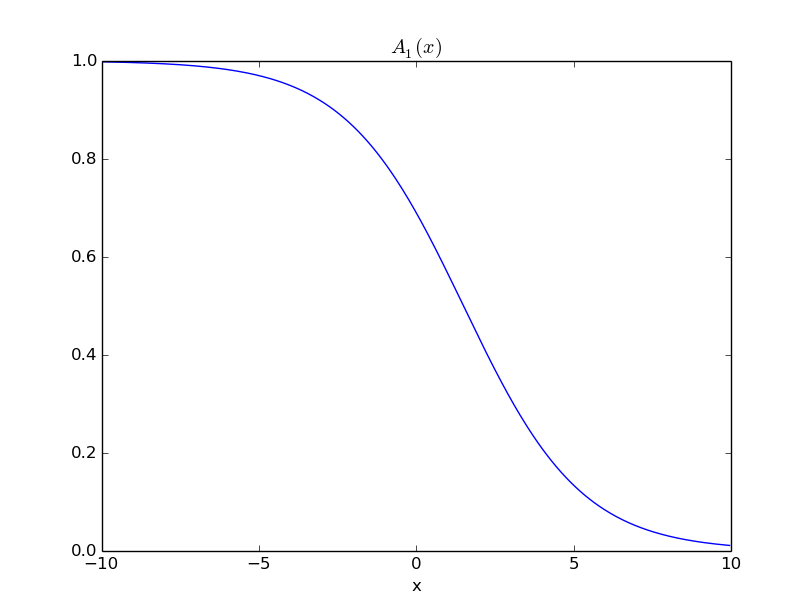
\includegraphics[width=\textwidth]{img/figure_1.png}
\end{subfigure}
\begin{subfigure}[b]{0.45\textwidth}
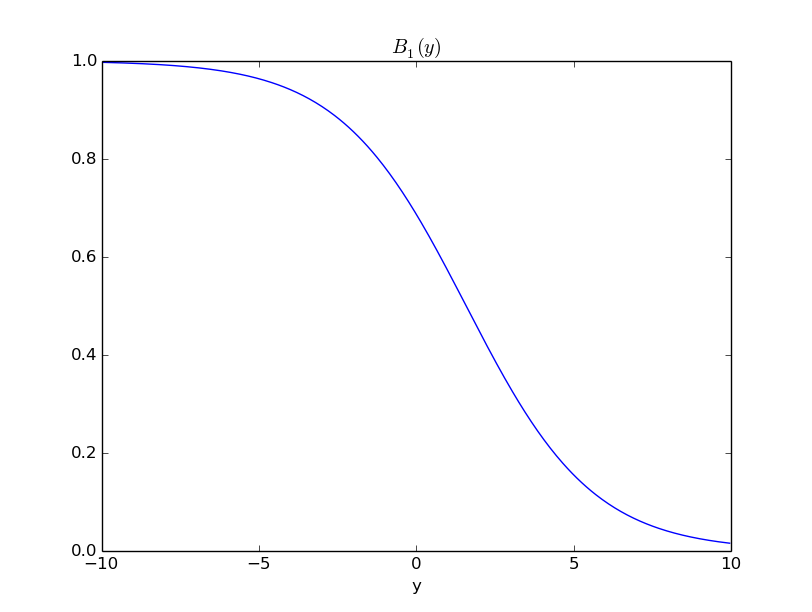
\includegraphics[width=\textwidth]{img/figure_2.png}
\end{subfigure}

\begin{subfigure}[b]{0.45\textwidth}
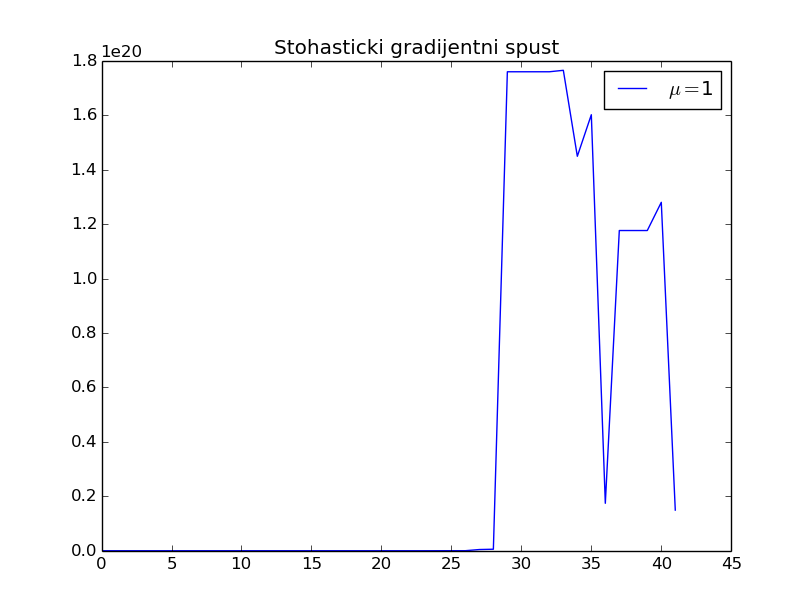
\includegraphics[width=\textwidth]{img/figure_3.png}
\end{subfigure}
\begin{subfigure}[b]{0.45\textwidth}
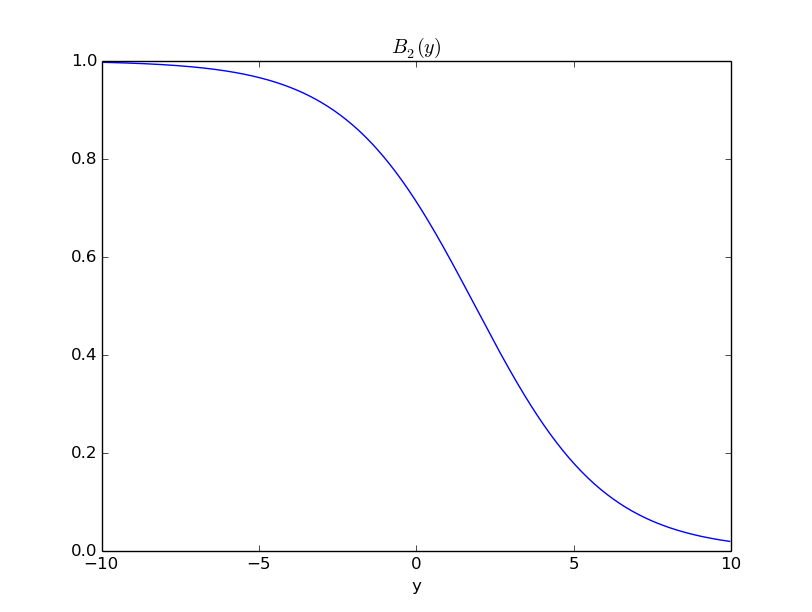
\includegraphics[width=\textwidth]{img/figure_4.png}
\end{subfigure}

\begin{subfigure}[b]{0.45\textwidth}
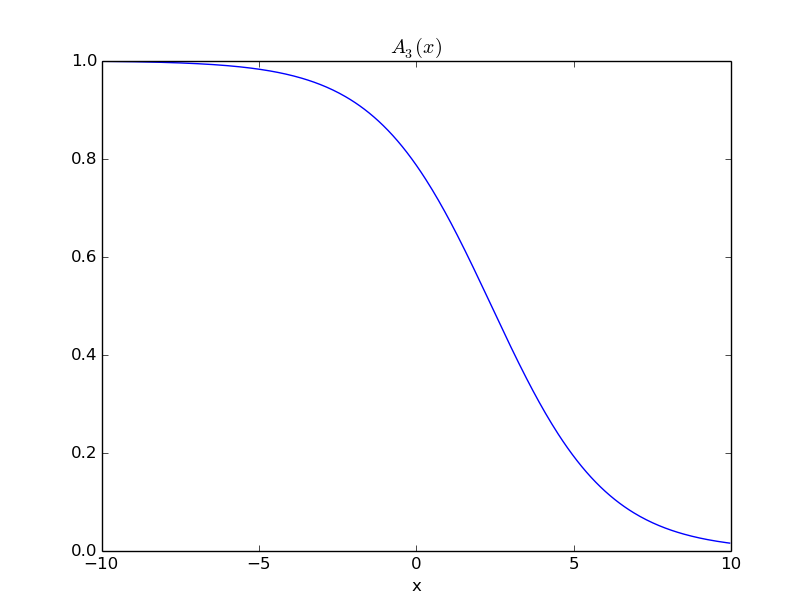
\includegraphics[width=\textwidth]{img/figure_5.png}
\end{subfigure}
\begin{subfigure}[b]{0.45\textwidth}
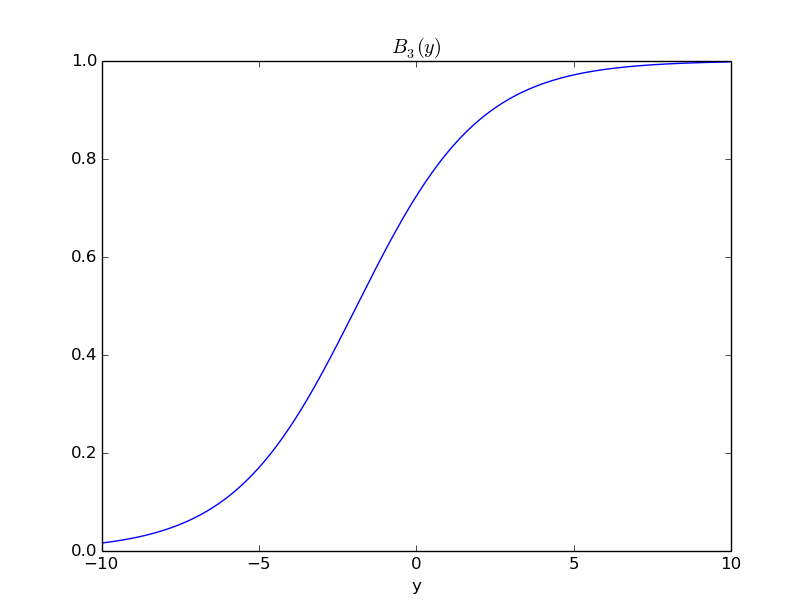
\includegraphics[width=\textwidth]{img/figure_6.png}
\end{subfigure}

\begin{subfigure}[b]{0.45\textwidth}
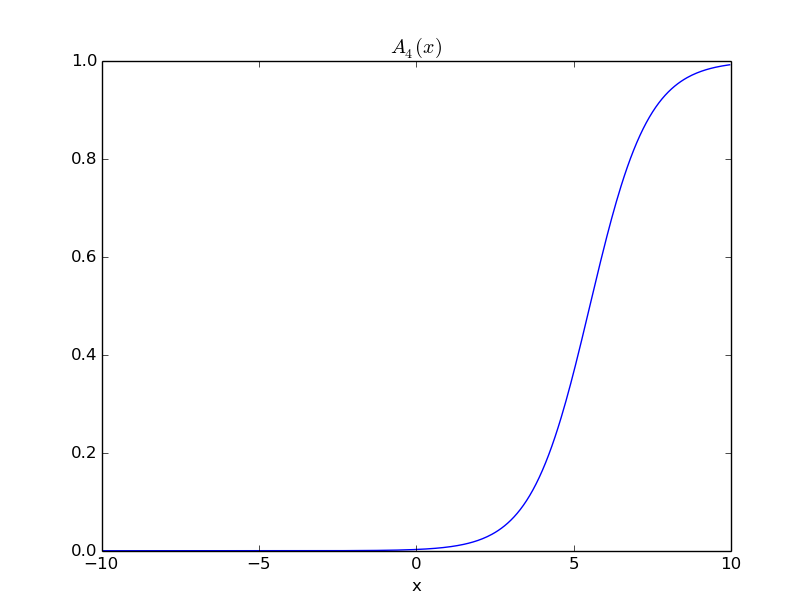
\includegraphics[width=\textwidth]{img/figure_7.png}
\end{subfigure}
\begin{subfigure}[b]{0.45\textwidth}
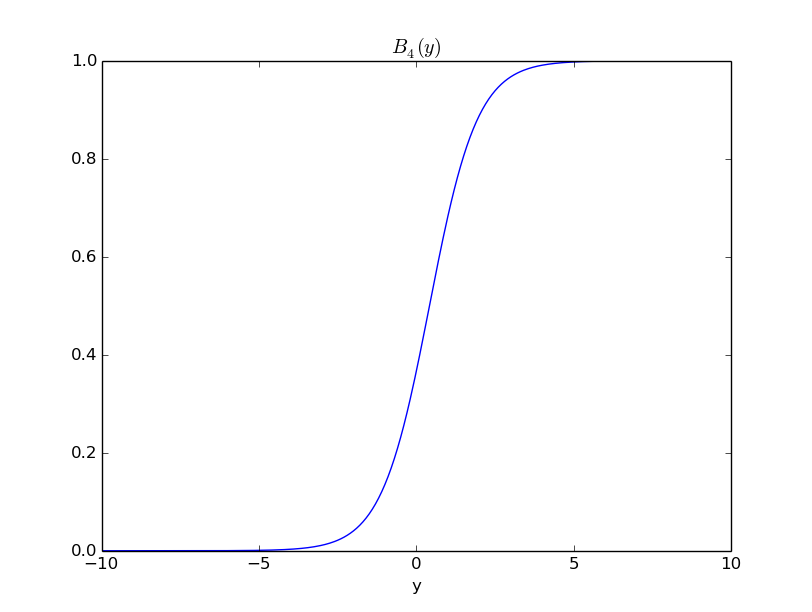
\includegraphics[width=\textwidth]{img/figure_8.png}
\end{subfigure}

\begin{subfigure}[b]{0.45\textwidth}
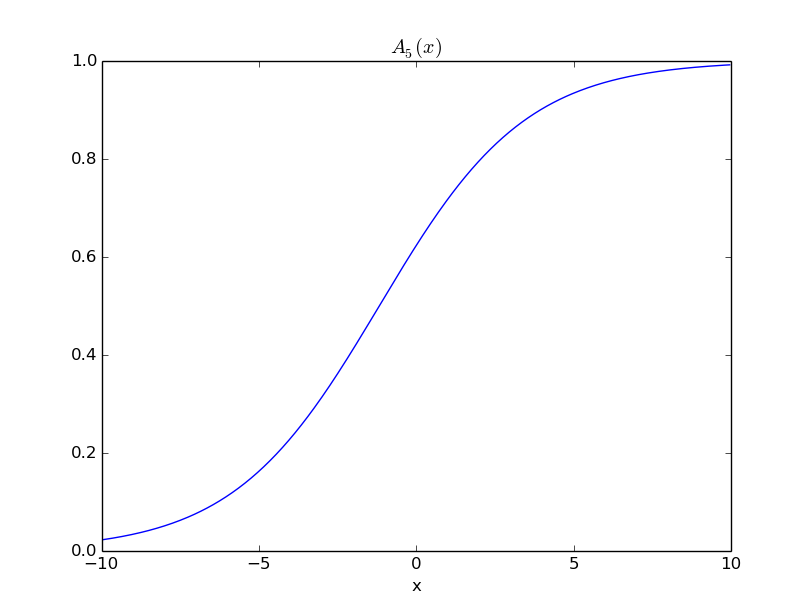
\includegraphics[width=\textwidth]{img/figure_9.png}
\end{subfigure}
\begin{subfigure}[b]{0.45\textwidth}
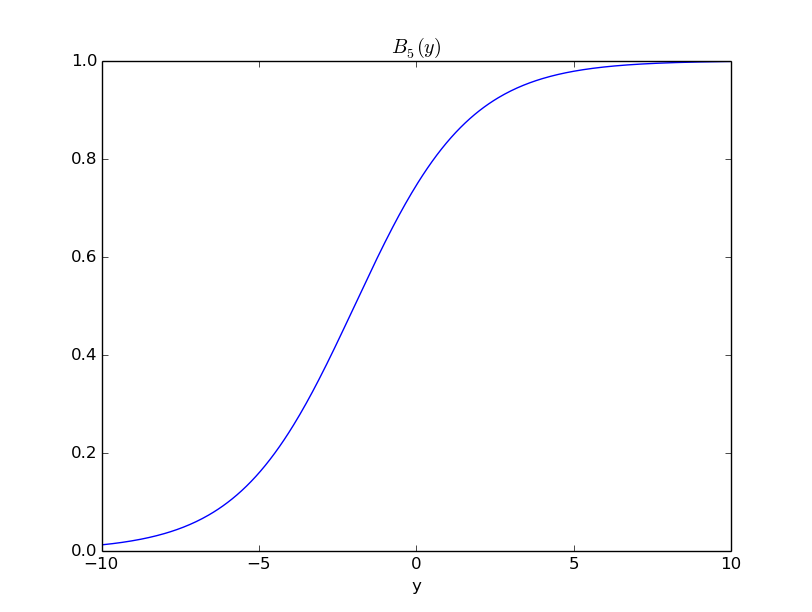
\includegraphics[width=\textwidth]{img/figure_10.png}
\end{subfigure}
\caption{Funkcije pripadnosti neizrazitih skupova $A_i$ i $B_i$ za svih $5$ pravila u bazi znanja. Funkcije su sigmoidalnog oblika. Primjetimo da se pojavljuju u svim mogućim kombinacijama rastućih i padajućih oblika.}
\end{figure}

\begin{figure}[h]
\begin{subfigure}[b]{0.5\textwidth}
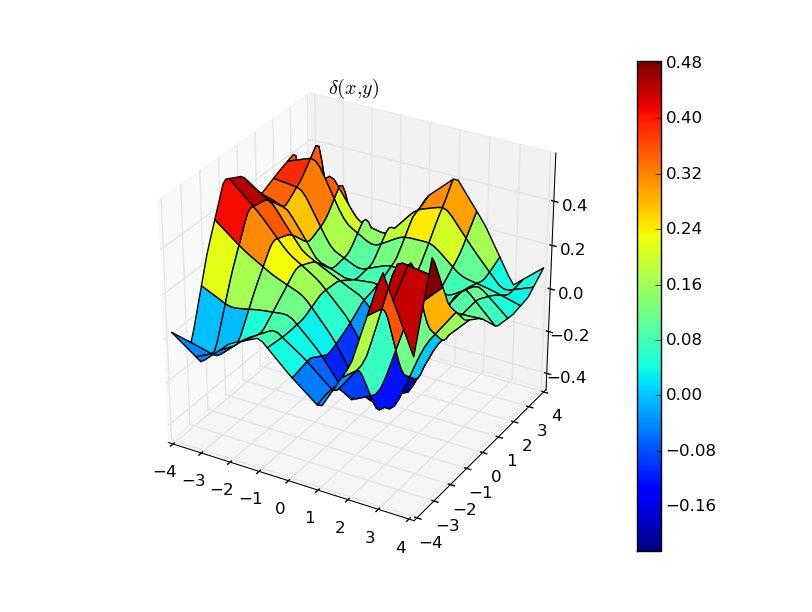
\includegraphics[width=\textwidth]{img/figure_zad6.png}
\end{subfigure}
\begin{subfigure}[b]{0.5\textwidth}
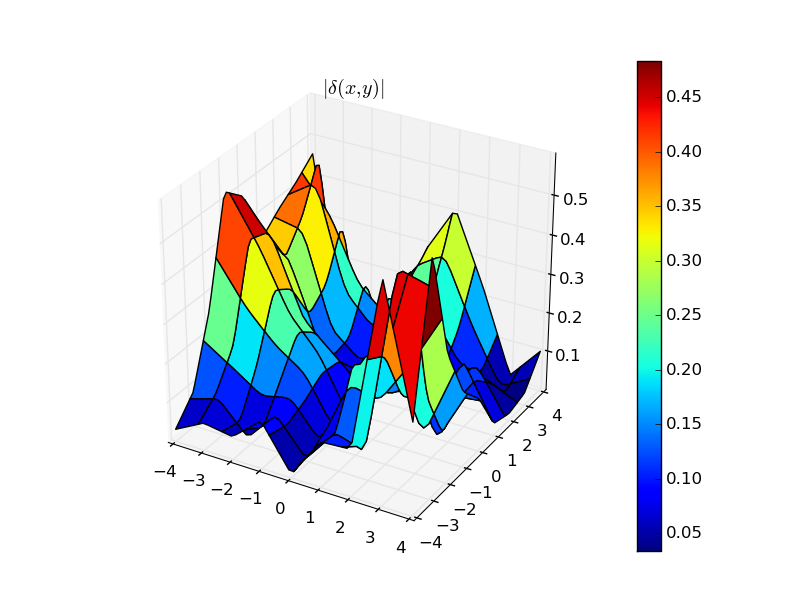
\includegraphics[width=\textwidth]{img/figure_zad6_2.png}
\end{subfigure}
\begin{subfigure}[b]{0.5\textwidth}
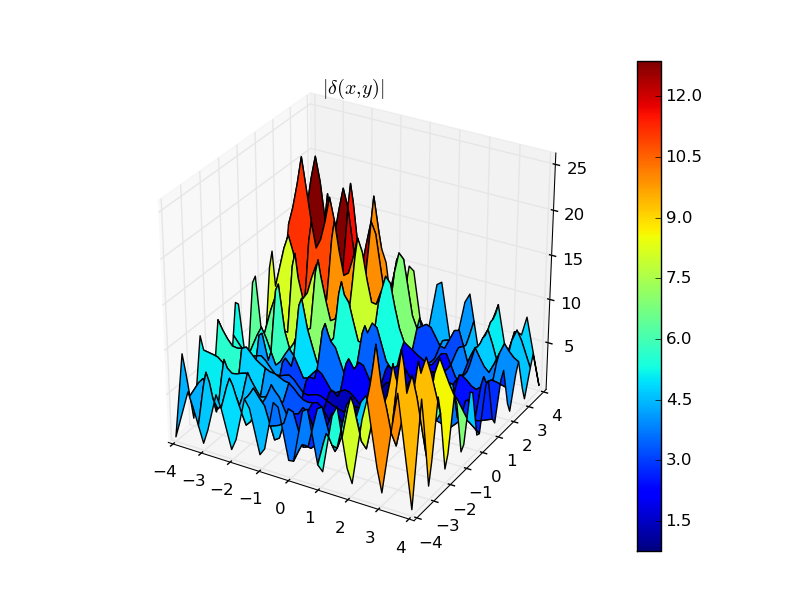
\includegraphics[width=\textwidth]{img/figure_zad6_3.png}
\end{subfigure}
\caption{Funkcija pogreške $\delta(x, y)$ za primjere iz skupa za učenje. }
\end{figure} 

\begin{figure}[h]
\centering
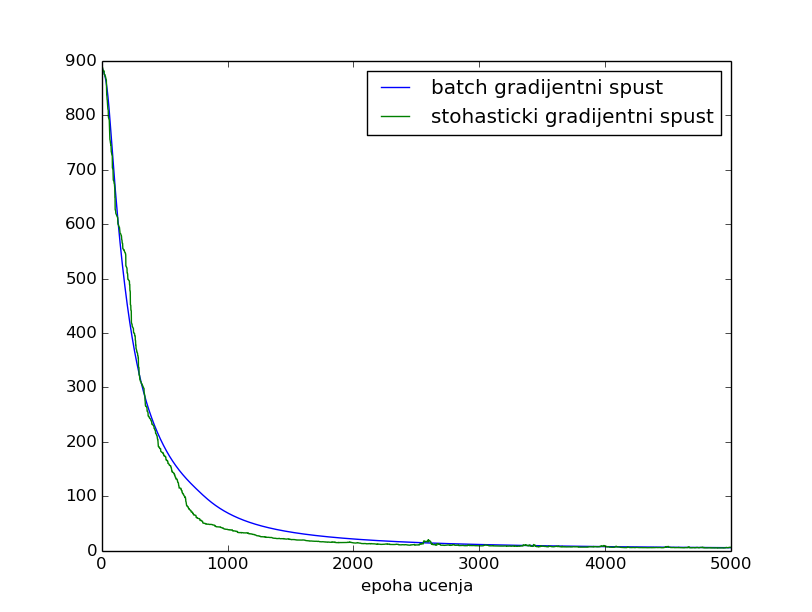
\includegraphics[width=0.8\textwidth]{img/figure_zad7.png}
\caption{Prosječna kvadratna pogreška na primjerima za učenje, $E$, po epohama učenja za obje verzije gradijentnog spusta. Dok je krivulja za batch verziju strogo padajuća, loše procjene gradijenta pogreške u stohastičkoj verziji uzrokuju česte lokalne maksimume funkcije pogreške, ali ipak uz globalni pad vrijednosti tijekom učenja.}
\end{figure}

\begin{figure}[h]
\centering
\begin{subfigure}[b]{0.7\textwidth}
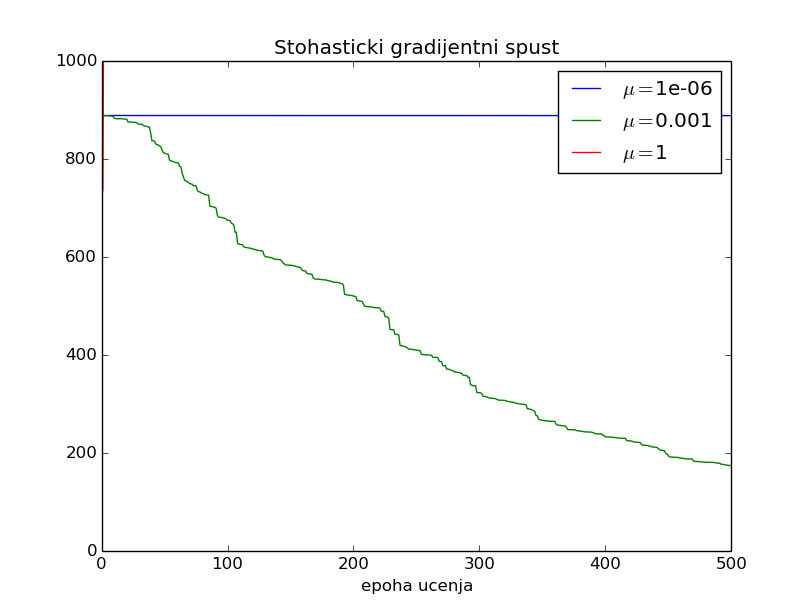
\includegraphics[width=\textwidth]{img/zad8_1.png}
\end{subfigure}
\begin{subfigure}[b]{0.7\textwidth}
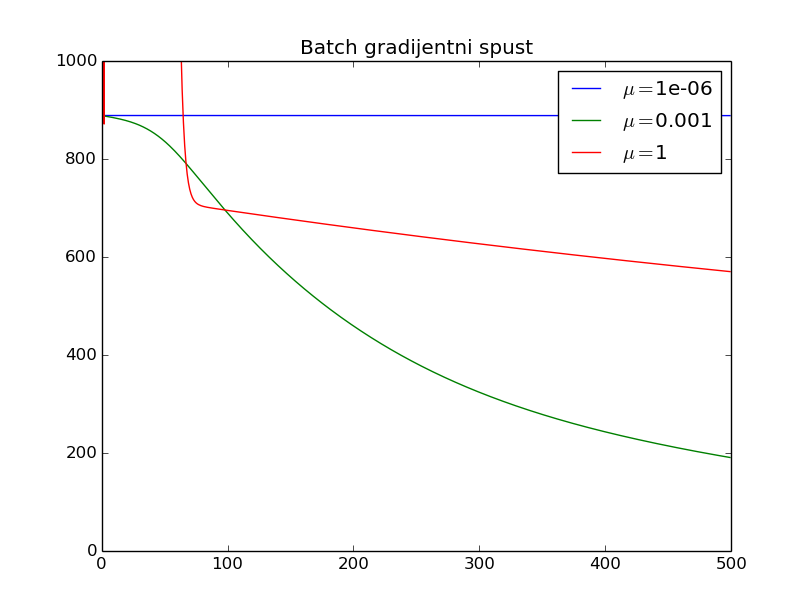
\includegraphics[width=\textwidth]{img/zad8_2.png}
\end{subfigure}
\caption{Pogreška učenja $E$ za obje verzije gradijentnog spusta uz stope učenja $\mu=\{10^{-6}, 10^{-3}, 1\}$.
Obje verzije gradijentnog spusta stagniraju za premalu stopu učenja $\mu=10^{-6}$.  Gradijentni spustovi za $\mu=10^{-3}$ konvergiraju. Stohastička verzija nema strogo padajuću krivulju zbog loših procjena gradijenata u samo jednoj točki, no takva joj procjena također pomaže u bržoj konvergenciji (i izlazasku iz lokalnih optimuma).
Batch verzija gradijentnog spustu za $\mu = 1$ divergira, dok za stohastičku verziju nakon nekoliko epoha pogreška kreće padati jer ju je procjena pogreške na temelju jednog primjera usmjerila izvan lokalnog optimuma.}
\end{figure}
\end{document}